\documentclass[titlepage,a4paper,12pt]{article}
% Indica el estilo que se va a usar para todo el documento.
% Parámetros:
% a4paper, letterpaper, a5paper, …
% landscape: Apaisado
% titlepage: Hace que el tıtulo y el resumen queden en una página aparte. El resumen se indica con la instrucción \abstract{..}
% 10pt, 11pt, 12pt, … Tamaño de la letra.
% twoside, oneside. Simple o doble faz.
% twocolumn. Texto a dos columnas.
%
% Clases de documentos:
% article: Informes pequeños, trabajos prácticos.
% report: Informes largos, tesis, guiones. Tiene capítulos y apartados.
% book
% slide: Diapositivas

%%%%%%%%%%%%%%%%%%%%%%%%%%%%%%%%
% Paquetes
%%%%%%%%%%%%%%%%%%%%%%%%%%%%%%%%
\usepackage{color} % Paquete para darle color a la sintaxis del codigo fuente.

% Establece los márgenes de la hoja, aunque los margenes por defecto son bastante buenos.
\usepackage[top=2cm, bottom=2cm, left=2cm, right=2cm]{geometry} 

\usepackage{latexsym} % Este paquete permite usar simbolos especiales, no relacionados con la matemática, como  \Join o \Box
\usepackage{verbatim} % Para escribir codigo fuente.
\usepackage{amsmath} % La gran mayoría de los simbolos matemáticos
\usepackage{amssymb} % Algunos pocos símbolos matemáticos más raros, como \digamma
\usepackage{siunitx} % Notación exponencial
\usepackage{pdfpages} % Importar PDF

\usepackage[spanish]{babel} % Definimos el documento como que esta en español.

\usepackage[utf8]{inputenx} % Este paquete permite usar los acentos y eñes directamente en el texto.

\usepackage{graphicx} % Para usar imagenes
\usepackage{float}
\usepackage{courier}
\usepackage{listings} % Paquete para importar código fuente.

\DeclareUnicodeCharacter{251C}{ }
\DeclareUnicodeCharacter{2500}{ }
\DeclareUnicodeCharacter{2514}{ }

% Con esta instrucción definimos el interlineado. Por defecto es 1.
\linespread{1}

% Con esta instrucción obtenemos el número de página en el pie y una cabecera con el nombre de la sección (o con la sección en las páginas pares y la subsección en las impares si hemos indicado la opción twoside en el comando documenclass).
%\pagestyle{headings}

% Pero también está la instrucción \pagestyle{myheadings}, que pone el número de página al pie y en la cabecera pone el texto especificado por los comandos ``markboth{...}{...}'' y ``markright{...}''.
\pagestyle{myheadings}
%\markboth{Encabezado izquierdo}{Encabezado derecho} % Para doble faz
\markright{Trabajo Práctico Final: Dune 2000} % Para una carilla.

% Si no hemos especificado la opción twoside, todas las páginas se consideran derechas. Podemos cambiar el estilo de la página en curso mediante \thispagestyle. Por ejemplo, si queremos que la página en curso no tenga número escribimos \thispagestyle{empty} en el cuerpo del documeento.

%%%%%%%%%%%%%%%%%%%%%%%%%%%%%%%%
% Portada
%%%%%%%%%%%%%%%%%%%%%%%%%%%%%%%%

% En la instrucción \title{..}, se escribe el título del documento.
\title{ Trabajo Práctico Final: Dune 2000 \\ 
 \large{Manual de Usuario}}

\author{Alvarez Juliá, Santiago \and Iglesias, Matias \and Sportelli Castro, Luciano}

% Aquí podemos escribir la fecha de realización del trabajo práctico. La fecha actual se escribe con \today. Si no se quiere incluir la fecha, dejar la instrucción en blanco.
\date{ \today }

%%%%%%%%%%%%%%%%%%%%%%%%%%%%%%%%%%%%%%%%%%%
% AQUI COMENZAMOS EL DOCUMENTO
%%%%%%%%%%%%%%%%%%%%%%%%%%%%%%%%%%%%%%%%%%%

\begin{document}

%Lo primero que hacemos es crear el titulo.
\maketitle

%Creamos los indices que sean necesarios.
\tableofcontents %Índice general
%\listoffigures %Indice de imágenes
%\listoftables %Indice de tablas

\newpage
\section{Instalación}
\subsection{Requisitos previos}
Bibliotecas:

\begin{itemize}
\item libsdl2-dev
\item libsdl2-image-dev
\item libsdl2-mixer-dev
\item libsdl2-ttf-dev
\item qt5-default
\end{itemize}

Utilidades:

\begin{itemize}
\item python3
\item 7z
\end{itemize}

\textbf{Archivos requeridos}

Para compilar el proyecto se debe crear una carpeta (comunmente denominada build) y se deben copiar dentro de la misma los archivos \texttt{sprites.7z} y \texttt{terrain.7z} provistos por la cátedra. Todos los archivos extra requeridos se encuentran en la carpeta data y serán copiados al lugar correspondiente por el instalador del juego.

Asumiendo que se compilará dentro de la carpeta build, la estructura debe quedar de la siguiente manera:

\begin{verbatim}
build/
├── sprites.7z
└── terrain.7z
\end{verbatim}

Observar que la carpeta build esta ignorada en el .gitignore.

El script de instalación se ocupará de descomprimir los mismos y copiarlos en la ubicación adecuada.

\subsection{Compilación e instalación}
Una vez creada la carpeta build y copiados los archivos terrain.7z y sprites.7z se debe proceder de la siguiente forma para compilar el proyecto.

\begin{verbatim}
~/tp-final-taller-1 $ cd build
~/tp-final-taller-1/build $ cmake -DCMAKE_INSTALL_PREFIX=./instalacion ..
~/tp-final-taller-1/build $ make
~/tp-final-taller-1/build $ make install
\end{verbatim}

El valor de \texttt{CMAKE\_INSTALL\_PREFIX} permite determinar donde se instalará el juego. Por defecto este directorio es \texttt{/usr/local}.

Opcionalmente se puede agregar a la variable de entorno PATH la ruta 

\begin{verbatim} 
<CMAKE_INSTALL_PREFIX>/bin 
\end{verbatim}

para poder ejecutar el mismo directamente.

\newpage
\section{Cliente}

\subsection{Ejecutar el programa}

Para ejecutar el cliente se debe ejecutar el siguiente comando:
\begin{verbatim}
$ dune-remake
\end{verbatim}

\subsection{Formas de uso}

Luego de ejecutar el cliente la primer ventana que verá es la siguiente:
\begin{figure}[H]
	\centering
	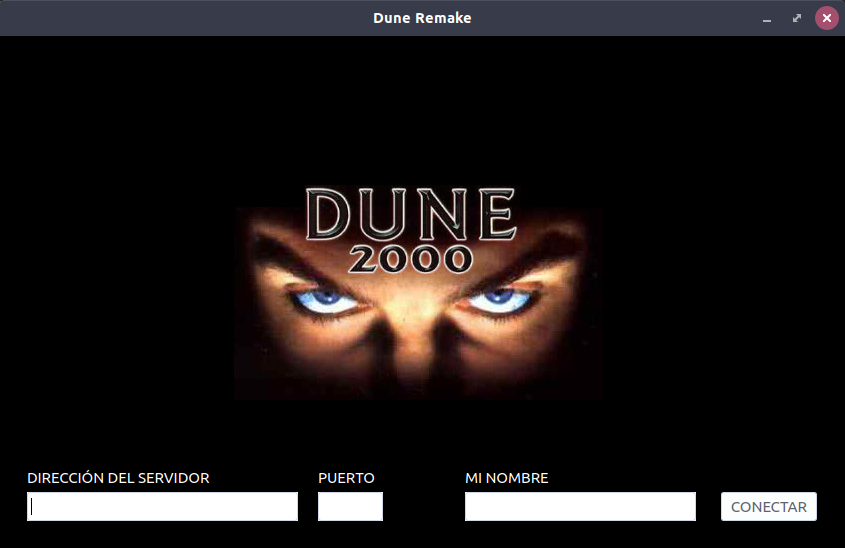
\includegraphics[width=12cm]{../imagenes/lanzador-cliente-conexion.png}
	\caption{\label{fig:lanzador-cliente-conexion} Pantalla de conexión.}
\end{figure}

Allí deberá ingresar los datos de conexión al servidor, es decir, la dirección y el puerto del mismo, y elegir un apodo que usará durante la partida.

Una vez conectado pasará a la sección elegir/crear sala:
\begin{figure}[H]
	\centering
	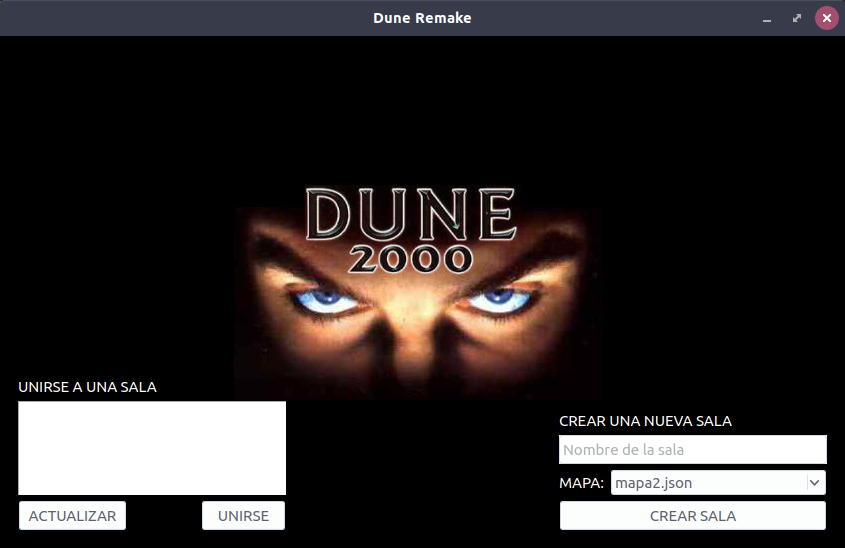
\includegraphics[width=12cm]{../imagenes/lanzador-cliente-elegir-sala.png}
	\caption{\label{fig:lanzador-cliente-elegir-sala} Pantalla de selección de sala.}
\end{figure}

En el panel de la izquierda verá las salas disponibles; puede hacer clic en actualizar para refrescar la lista de salas. En el panel de la derecha verá una lista con los mapas disponibles y podrá crear una nueva sala.

Al haber elegido una sala o creado una, pasará a la sección ``en sala'' que se verá de la siguiente forma:
\begin{figure}[H]
	\centering
	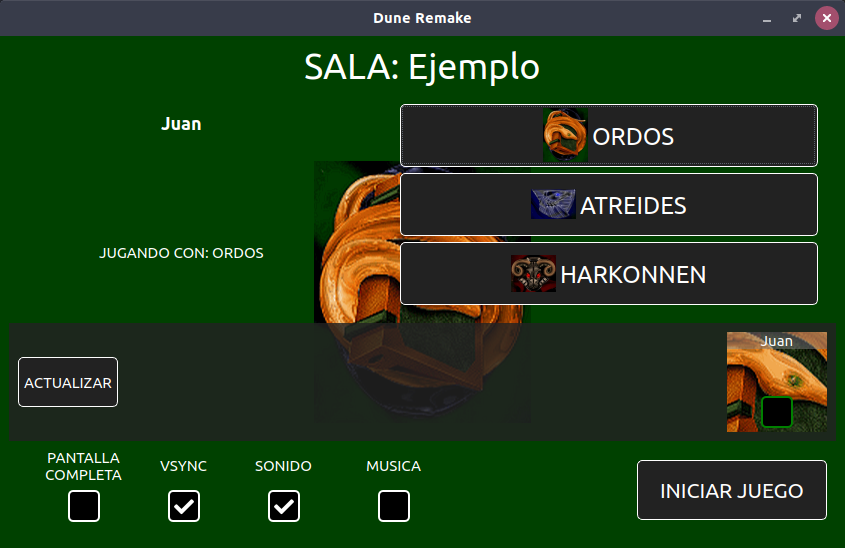
\includegraphics[width=12cm]{../imagenes/lanzador-cliente-en-sala.png}
	\caption{\label{fig:lanzador-cliente-en-sala} Pantalla previa al juego.}
\end{figure}

En esta pantalla deberá elegir con qué casa jugar, haciendo clic en los botones de arriba a la derecha (Atreides, Harkonnen u Ordos). Una vez elegido podrá ver en el panel del medio al resto de los jugadores conectados. La lista se actualizará automáticamente cada 10 segundos pero puede forzar la actualización haciendo clic en el botón actualizar.

En la sección inferior puede configurar distintas opciones del juego, como la pantalla completa, el sincronismo vertical, la música y los sonidos. 

Si el sincronismo vertical está activo, la actualización de la pantalla de juego se hará coincidir con el refresco del monitor; si está inactivo se fijarán las actualizaciones de la ventana no más que 30 cuadros por segundo.

Cuando haya terminado de elegir y configurar el juego, y todos los jugadores ya estén en la sala puede pulsar Iniciar Juego para iniciar la partida. Cabe destacar que en el momento en que uno de los jugadores pulse Iniciar Juego la sala se cerrará y se esperará a que el resto de los jugadores inicie la partida. Es por esto que deben estar todos dentro de la sala antes de que alguno dé inicio a la partida.

En este momento comenzará a ejecutarse el juego. Verá unos instantes una pantalla informandole la espera de todos los jugadores y luego pasará a la ventana de juego:
\begin{figure}[H]
	\centering
	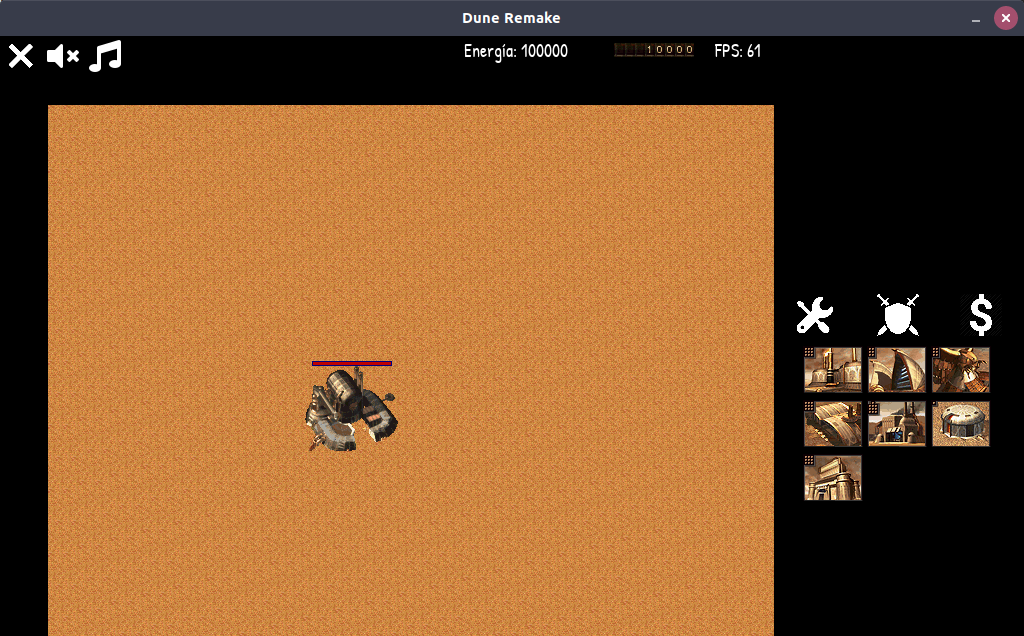
\includegraphics[width=16cm]{../imagenes/cliente-en-partida.png}
	\caption{\label{fig:cliente-en-partida} Ventana de juego.}
\end{figure}

La ventana de juego se compone de tres secciones: la barra superior, el panel lateral y el área de juego. 

En la barra superior encontrará a la izquierda tres botones que le permitiran salir del juego (la cruz), y activar o desactivar los sonidos y la música. A la derecha de la misma encontrará la energía y el dinero disponible, y los cuadros por segundo a los que se está reproduciendo el juego.

En el panel lateral se encuentran las acciones de juego, puede elegir construir edificios haciendo clic en el ícono de la llave; entrenar tropas haciendo clic en el ícono del escudo o vender un edificio haciendo clic en el ícono de pesos. Al iniciar la construcción de un edificio verá en sobre el botón el tiempo faltante para la construcción. Puede volver a hacer clic para encolar otra construcción del mismo tipo o hacer clic sobre un botón de otro edificio para iniciar otra construcción. Análogamente sucede con los entrenamientos. Debe tener en consideración que para poder entrenar tropas requiere tener ciertos edificios construidos. Para cancelar una construcción o entrenamiento (eliminarlo de la cola), haga clic con el botón derecho sobre el entrenamiento o construcción que quiera cancelar. Sólo se pueden cancelar encolados, los que están en curso no podrán ser cancelados.

Una vez que un edificio se termine de construir el botón del mismo se tornará verde. Esto indica que está listo para ser ubicado. Para ubicar el edificio en el terreno, haga clic izquierdo en el boton y luego haga clic izquierdo en el lugar del mapa en el que desee ubicarlo. Sólo puede ubicar un edificio si el terreno lo permite y si está a 5 casillas o menos de otro edificio.

En el área de juego es donde sucede la acción. Ahí vera sus edificios y tropas y los de los rivales. Desde aquí puede seleccionar tropas e indicarles hacia donde dirigirse o a quién atacar y moverse sobre el terreno. Para seleccionar tropas, haga clic izquierdo sobre un punto y arrastre el mouse para crear un rectángulo que contenga a las tropa sque quiera seleccionar. Puede mantener apretado CTRL y realizar otra selección para seleccionar tropas que estén en distintos lugares. 

Teniendo tropas seleccionadas puede hacer clic derecho sobre el terreno para indicarles que deben moverse a esa ubicación o sobre una unidad o edificio enemigo para indicarles que ataquen.

Para centrar la cámara en su centro de construcciones puede pulsar la tecla F2.



\newpage
\section{Servidor}

\subsection{Ejecutar el programa}

Para ejecutar el servidor del juego, una vez instalado deberá correr el siguiente comando:
\begin{verbatim}
$ dune-remake-servidor
\end{verbatim}

Una vez ejecutado el servidor cargará la configuración desde el archivo \texttt{config.json}, que se ubica en \texttt{\{prefijo de instalacion\}/etc/dune-remake/config.json}. Usualmente esto es \texttt{/usr/local/etc/dune-remake/config.json}.

A partir de este archivo se cargarán los mapas disponibles, la información sobre edificios y ejércitos y se escucharán conexiones en el puerto establecido.

Opcionalmente, se puede pasar como argumento de línea de comandos la opción \texttt{-c <archivo>} para cargar un archivo de configuración en una ubicación específica, o la opción \texttt{-p <puerto>} para escuchar en un puerto distinto al indicado en el archivo de configuración.

Al iniciarse el servidor mostrará desde donde está cargando el archivo de configuración, los mapas disponibles y en que puerto escuchará conexiones. Para cerrar el servidor ingrese la letra `q'.

Ejemplo de ejecución:
\begin{verbatim}
$ ./dune-remake-servidor
Configuración cargada desde /etc/dune-remake/config.json
Información de edificios tomada desde: /etc/dune-remake/edificios.json
Información de tropas tomada desde: /etc/dune-remake/ejercitos.json
Mapas cargados: 
	/etc/dune-remake/mapas/mapa-1.json
	/etc/dune-remake/mapas/mapa-4-jugadores.json
	/etc/dune-remake/mapas/mapa-arrakis.json
Escuchando en el puerto: 9432
Ingrese 'q' para salir
Esperando conexiones...
q
Deteniendo el servidor... Esto puede llevar un tiempo.
Se detuvo el servidor
\end{verbatim}

\newpage
\section{Editor}

\subsection{Ejecutar el programa}

Para ejecutar el cliente se debe ejecutar el siguiente comando:
\begin{verbatim}
$ dune-remake-editor
\end{verbatim}

\subsection{Formas de uso}

El editor de mapas puede ser utilizado de 2 formas diferentes, para crear mapas y para cargar mapas para poder editarlos. La siguiente captura de pantalla pertenece al dialogo de bienvenidad del programa. En el se puede elegir entre crear un mapa desde cero o cargar un mapa ya manipulado, almacenado en la computadora.

\begin{figure}[H]
	\centering
	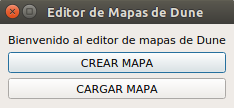
\includegraphics[width=0.25\textwidth]{../imagenes/bienvenida_editor.png}
	\caption{\label{fig:menu_editor} Dialogo de bienvenida del editor.}
\end{figure}

\subsubsection{Crear mapa}

Para crear un mapa nuevo, hay que presionar el botón 'Crear mapa' del dialogo de bienvenida, lo que genera una ventana de configuración en la que deben ser elegidos el tamaño del mapa y la cantidad de jugadores. La dimensión mínima del mapa es de 20x20 celdas y la cantidad de jugadores mínima es 2. \\

\begin{figure}[H]
	\centering
	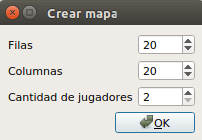
\includegraphics[width=0.25\textwidth]{../imagenes/conf_nuevo_mapa.png}
	\caption{\label{fig:menu_editor} Configuración nuevo mapa.}
\end{figure}

Luego de completar la configuración del mapa, se abrirá el editor de mapas en sí mismo. Esta compuesto por 3 elementos: el mapa, la pestaña con los terrenos que pueden ser ubicados en el mapa y la barra de menu.\\

\begin{figure}[H]
	\centering
	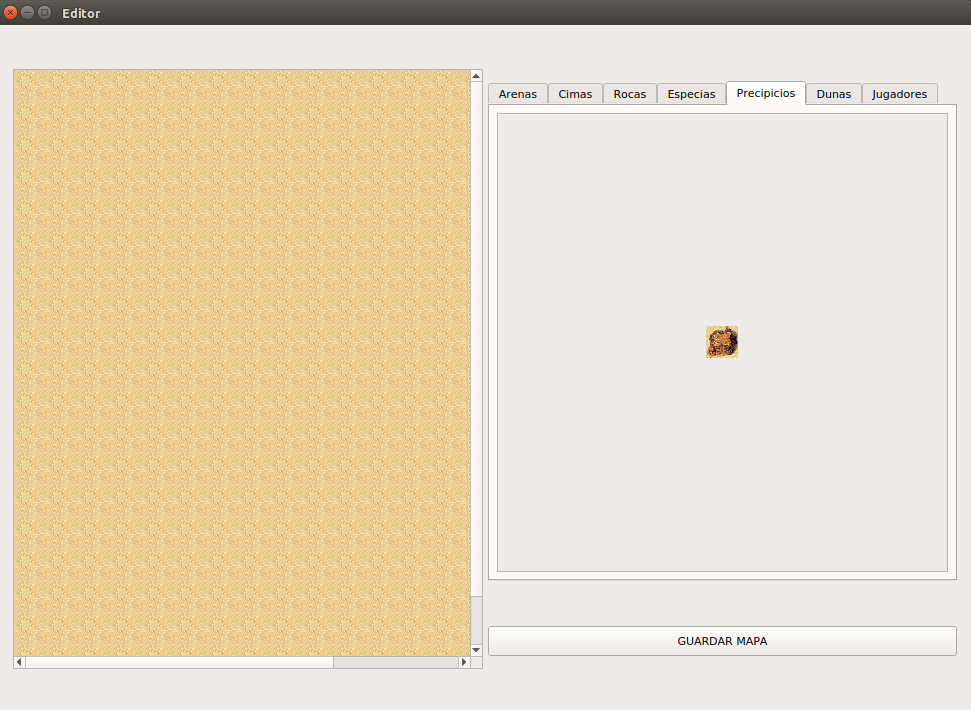
\includegraphics[width=0.75\textwidth]{../imagenes/editor_ui.png}
	\caption{\label{fig:menu_editor} Editor.}
\end{figure}

\subsubsection{Cargar mapa}

Para crear un mapa nuevo, hay que presionar el botón 'Crear mapa', lo que genera una nueva ventana para elegir el archivo del mapa.\\

\begin{figure}[H]
	\centering
	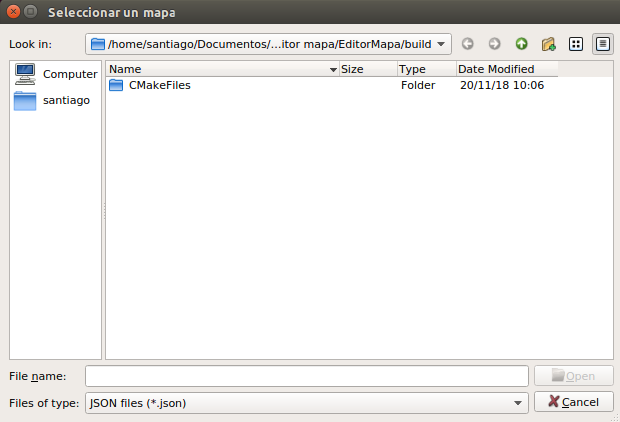
\includegraphics[width=0.6\textwidth]{../imagenes/cargar_mapa.png}
	\caption{\label{fig:menu_editor} Cargar mapa.}
\end{figure}

Luego de seleccionar el archivo se abrirá la ventana del editor en sí mismo, al igual que al crear un mapa nuevo.\\

\subsubsection{Agregar un terreno al mapa}

En la pestaña Terrenos se encuentran todos los terrenos que pueden ser agregados al mapa. Para agregar un terreno al map, seleccionarlo haciendo click izquierdo sobre el tile (se podrá ver un marco negro sobre el terreno seleccionado). Luego mover el mouse hacia el lugar del mapa sobre el que quiere agregarse el terreno, se podrá ver también un marco negro sobre el terreno del mapa que va a ser reemplazado. Finalmente hacer click izquierdo sobre el tile del mapa para reemplazarlo por el seleccionado en la pestaña.

\subsubsection{Editar configuración del mapa}

En todo momento puede cambiarse la configuración del mapa que fue seleccionada al crearlo. En el menu Editar aparecen 2 opciones, cambiar cantidad de jugadores y cambiar tamaño del mapa. Al seleccionarlas, aparecerá un dialogo para poder editar dichas configuraciones. En ambos casos se muestra en el dialogo la configuración elegida anteriormente.\\

\begin{figure}[H]
	\centering
	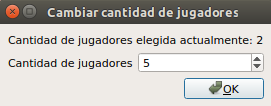
\includegraphics[width=0.6\textwidth]{../imagenes/cambiar_jugadores.png}
	\caption{\label{fig:menu_editor} Cambiar cantidad de jugadores.}
\end{figure}

La cantidad de jugadores siempre va a ser mínimo 2 y en el caso de que ya haber agregado jugadores al mapa (y estos sean mas que 2), el mínimo de cantidad de jugadores pasa a ser la cantidad de jugadores agregados.\\

\begin{figure}[H]
	\centering
	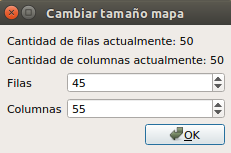
\includegraphics[width=0.6\textwidth]{../imagenes/cambiar_tamanio.png}
	\caption{\label{fig:menu_editor} Cambiar tamaño del mapa.}
\end{figure}

Al cambiar el tamaño del mapa debe tenerse en cuenta que la fila 0 y la columna 0 se encuentran en la parte superior izquierda del mapa.\\

\subsubsection{Guardar mapa}

Para guardar el mapa dirigirse al menú Archivo y seleccionar la opción 'Guardar mapa'. Tener en cuenta que antes deben haberse agregado al mapa la cantidad de jugadores indicadas por el usuario, en caso contrario se visualizará un mensaje de error. Se abrirá una ventana para seleccionar el directorio del mapa y su nombre (puede incluir o no la extensión del archivo .json). En el caso de que ya exista un mapa con el mismo nombre en el mismo directorio, este será sobreescrito.

\subsubsection{Cargar mapa desde el Editor}

Además de poder cargar un mapa en el dialogo de bienvenida también se puede cargar un mapa luego de iniciado el Editor. En el menú 'Archivo' seleccionar la opción 'Cargar mapa'. Tener en cuenta que al cargar un mapa, se perderá el progreso del mapa que se estaba editando hasta ese momento.

\subsection{Errores al utilizar el programa}

Es posible que aparezcan mensajes de error al utilizar el editor. Estos errores aparecen cuando el usuario quiere realizar una acción prohibida por el programa, como por ejemplo, agregar un jugador sobre la arena. En ese caso en particular, el mensaje de error aclara que los jugadores solo pueden ser ubicados sobre la roca. En todos estos casos el mensaje de error es extremadamente descriptivo.

\end{document}
